 \section*{Ziel}
    Es soll die Güteziffer $\nu$ einer Wärmepumpe, der Massendurchsatz 
    von Dichlordifluormethan $Cl_2F_2C$ und die mechanische Leistung des verwendeten
    Kompressors ermittelt werden.
\section{Theorie}  
\label{sec:theorie}
    Natürlicherweiße fließt Wärmeenergie in einem abgeschlossenen
    System von einem heißen immer ins kalte Reservoir.
    Möchte man den Wärmefluss umkehren, so muss Arbeit verrichtet werden.
    Diese Aufgabe übernimmt eine sogenannte Wärmepumpe.\\
    Es gilt nach dem ersten Hauptsatz der Theromdynamik:
    \begin{equation}
        Q_1=Q_2+A
        \label{eqn:1HS}
    \end{equation}
    Für das Verhältnis der Wärmemenge $Q$ und der Temperatur $T$ bei reversiblen
    Wärmeübertragungen gilt nach dem zweiten Hauptsatz:
    \begin{equation}
        \frac{Q_1}{T_1}-\frac{Q_2}{T_2}=0
        \label{eqn:2HS}
    \end{equation}
    Da ein vollständige reversible Umwandlung in der realen Umsetzung 
    nicht möglich ist gilt:
    \begin{equation*}
        \frac{Q_1}{T_1}-\frac{Q_2}{T_2}>0
    \end{equation*}\\

    Die Güteziffer einer Wärmepumpe ist definiert als 
    \begin{equation}
        \nu=\frac{Q_1}{A}
        \label{eqn:v_main}
    \end{equation}
    somit folgt mit Gleichung \eqref{eqn:1HS}, \eqref{eqn:2HS} und \eqref{eqn:v_main}:
    \begin{equation}
        \nu_{ideal}=\frac{Q_1}{A}=\frac{T_1}{T_1-T_2}>\nu_{real}
        \label{eqn:nu_ideal}
    \end{equation}

Die reale Güteziffer ergibt sich nach:
    
    \begin{equation}
        \nu_{real}=\frac{\Delta Q_1}{\Delta tN}=(m_2c_w + m_kc_k)\;\frac{\Delta T_2}{\Delta tN}=L\frac{\Delta m}{\Delta tN}     
    \end{equation}
        
    Dabei ist $N$ die über die Zeit $\Delta t$ gemittelte Leistungsaufnahme des Kompressors, $m$
    der Massendurchsatz und $L$ die Verdampfungswärme.

%selbstziterung weil wir geil sind    
\subsection*{Verdampfungswärme $L$}
Die Dampfdruckkurve wird bestimmt durch die Verdampfungswärme $L$.
Diese Größe ist eine charakteristische Größe der Substanz und im allgemeinen temperaturabhängig.
\uline{Definition molare Verdampfungswärme $L$:}
\begin{flushleft}
Gibt die Enerie an, die benötigt wird, um einen Mol einer Flüssigkeit in Dampf
der gleichen Temperatur umzuwandeln. 
\cite{Verdampfungswärme}[4]
\end{flushleft}




\subsection*{Mechanische Kompressionsleistung}
Für die machanische Kompressionsleistung $N_{mech}$ gilt:
\begin{gather}
    A_m=-p_av_a^{\kappa}\int_{v_a}^{v_b} V^{-\kappa}dV=\frac{1}{\kappa -1}p_aV_a^{\kappa}(V_b^{-\kappa +1}-V_a^{-\kappa+1})=\frac{1}{\kappa-1}(p_b\sqrt[\kappa]{\frac{p_a}{p_b}}-p_a) V_a \label{eqn:kompress} \\
    N_{mech}=\frac{\Delta A_m}{\Delta t}=\frac{1}{\kappa -1}(p_b\sqrt[\kappa]{\frac{p_a}{p_b}}-p_a)\frac{\Delta V_A}{\Delta t}=\frac{1}{\kappa -1}(p_b\sqrt[\kappa]{\frac{p_a}{p_b}}-p_a)\frac{1}{\rho}\frac{\Delta m}{\Delta t}\label{eqn:kompress2}
\end{gather}
wobei $\rho$ die Dichte des Gases beschreibt und $p_a$ den Druck.



\subsection*{Wärmepumpe}
Nun soll die Funktionsweise der Wärmepumpe erörtert werden.
Diese verwendet ein reales Gas, welches beim phasen Wärmeenergie umwandel, hier also beim Verdampfen Wärme 
aufnimmt und diese beim Verflüssigen wieder abgiebt.
Dabei wird ein Gas mit einer möglichst hohen Kondensationswärme verwendet.
Der generelle Aufbau ist dabei in Abbildung \ref{fig:aufbau_generell} gezeigt.
\begin{figure}[H]
    \centering
    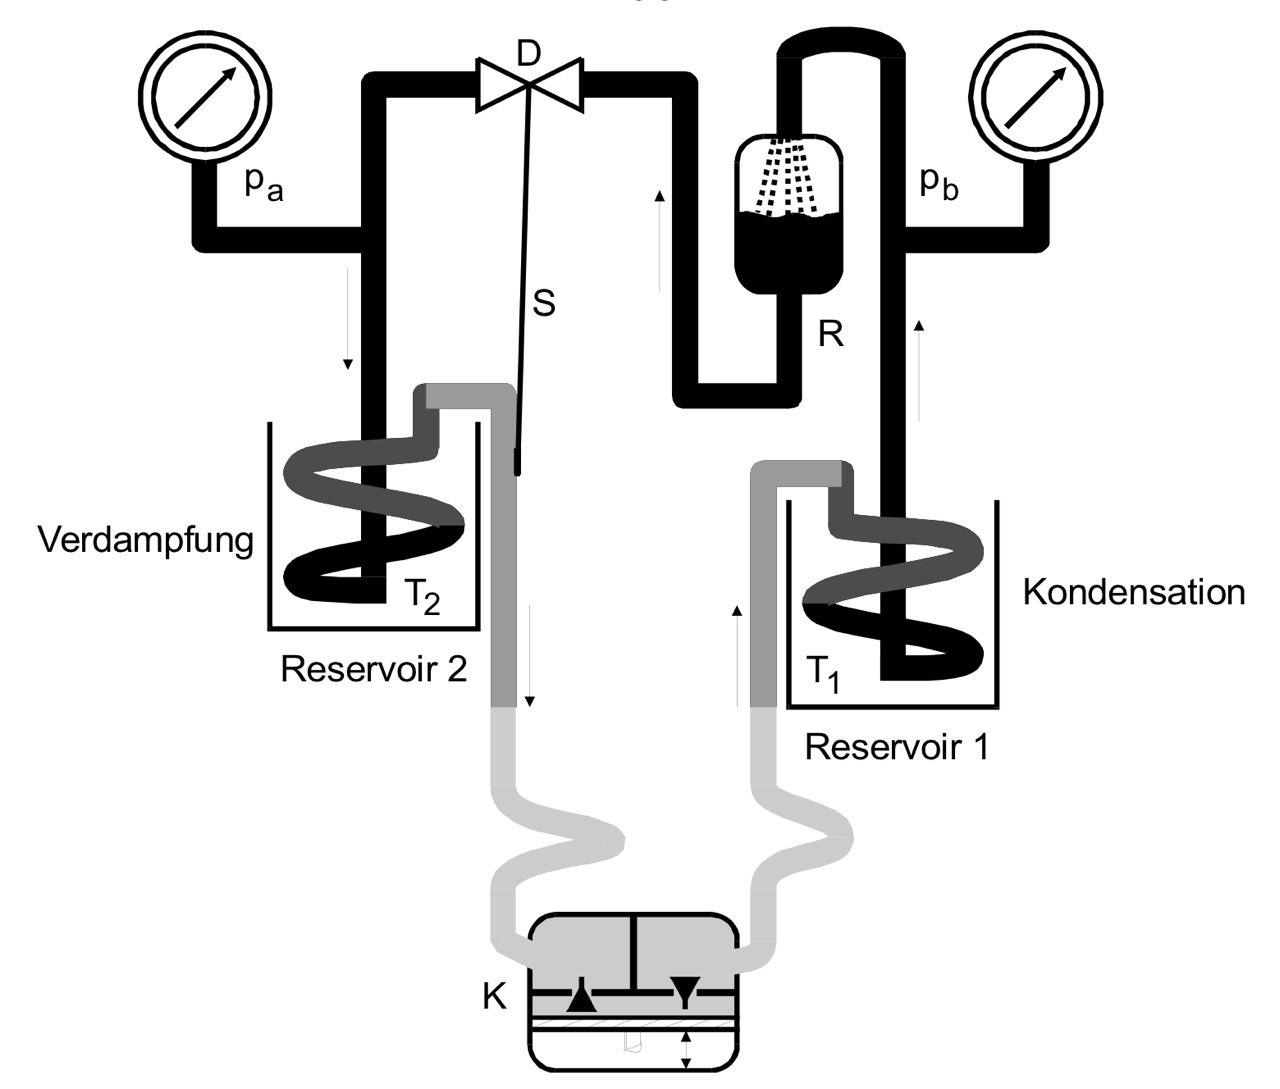
\includegraphics[width=0.5\textwidth]{bilder/aufbau_generell.jpg}
    \caption{Genereller Aufbau der Wärmepumpe \cite[196]{Anleitung}}
    \label{fig:aufbau_generell}
\end{figure}
Der dargestellte Kompressor $K$ leistet dabei die nötige Arbeit und 
erzeugt dabei einen Mediumkreislauf. Für die Druckzonen
der Reservoire 1 und 2 sorgt das Drosselventil $D$.
Dieses verfügt über eine Steuereinheit, sodass die Ventielöffnung
anhand der Temperaturdifferenz der beiden Reservoire geregelt werden kann.\\

Genauer, wird in dem Reservoire 1 das Medium bei einem Druck von $p_1$ kondensiert, dass heißt, das Medium gibt Wärmeenergie
ab und somit nimmt die Wasser Temperatur $T_1$ zu.
Nachdem das Druckventil $D$ durchlaufen wurde verdampft das Medium bei einem Druck von $p_2$ und nimmt dabei Wärmeenergie auf,
wodurch die Temperatur $T_2$ im Reservoire 2 abnimmt.

Um einen Reibungsfeien Ablauf zu der Anlage gewärhleisten, sind
im Kreislauf noch weiter Aperaturen eingebaut, die allerdings die funktionsweise
nicht weiter verändern.\\
In der Abbildung ist beispielsweise ein "Reiniger" $R$ dargestellt, um 
das Kondensierte Medium von Gas-Blasen zu befreien.  


